%TODO zweryfikować ten dokument jak już zaktualizują ubuntu.com
%obrazek
%linki
%rozmiar obrazów instalacyjnych
\begin{center}
	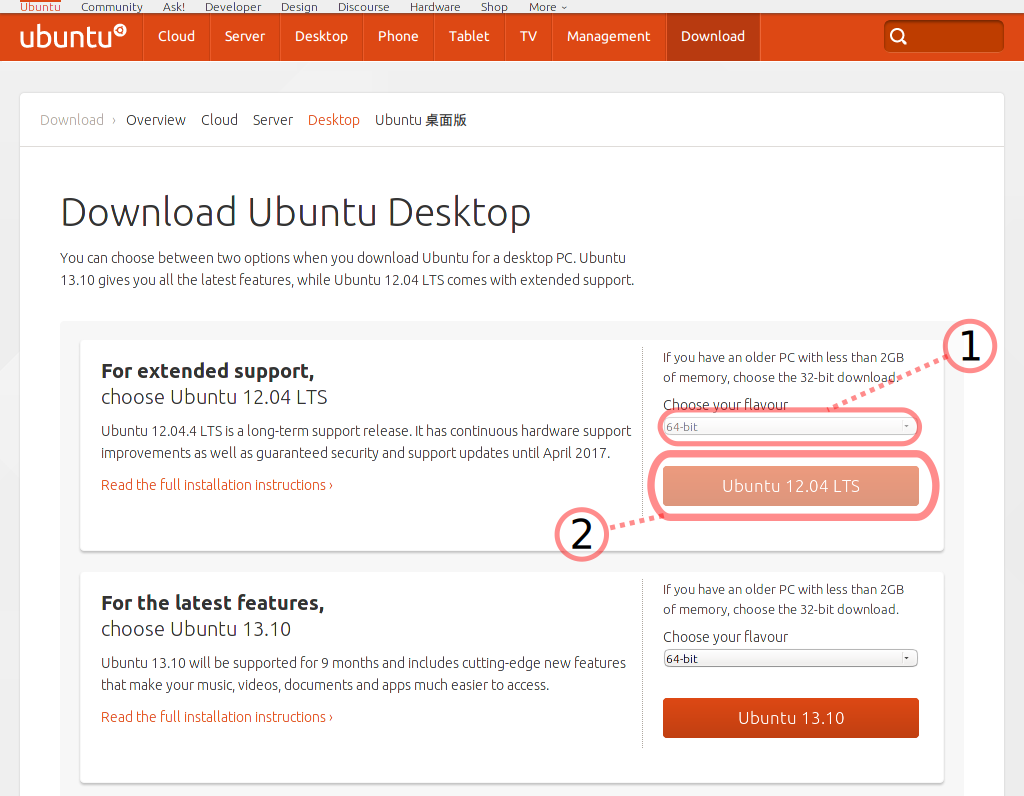
\includegraphics[width=\linewidth]{images/instalacja_pobieranie_obrazu.png}
\end{center}

Pierwszym etapem instalacji systemu jest pobranie instalatora. W tym celu udaj się na stronę \href{http://www.ubuntu.com/download/desktop}{ubuntu.com} i z górnego paska wybierz \textcolor{ubuntu_orange}{Download}, a następnie \textcolor{ubuntu_orange}{Desktop}.
\begin{enumerate}[label=\protect\circled{\arabic*}]
\item To pole pozwoli ci wybrać pomiędzy 32- a 64-bitową wersją systemu. Domyślnie wybrana jest wersja 64-bitowa.
\item Kliknij ten przycisk, aby przejść dalej.
\end{enumerate}

Następnie będziesz mieć możliwość przekazania dotacji na rzecz Ubuntu. Nie będziemy się tym teraz zajmować. Przewiń stronę w dół i kliknij \textcolor{ubuntu_orange}{Not now, take me to the download}. Zostaniesz przeniesiony na kolejną stronę, a po kilku sekundach rozpocznie się pobieranie obrazu systemu.

Jeżeli twój komputer został wyprodukowany nie dawnej niż 5 lat temu, wersja 64-bitowa będzie na pewno odpowiednia. Jeżeli masz mniej niż 2 gigabajty RAM-u, wybierz wariant 32-bitowy. Niezależnie od tego, jaką wersję wybierzesz, i tak będziesz mieć dostęp do takiego samego zestawu oprogramowania. Wariant 64-bitowy jest lepiej dopasowany do nowoczesnych komputerów, jeżeli jednak masz jakiekolwiek wątpliwości, wybierz wersję 32-bitową. Będzie ona działać także na 64-bitowym komputerze, choć nie będzie wykorzystywać wszystkich jego możliwości.
Jeżeli twoja płyta główna kontrolowana jest przez UEFI, musisz wybrać system 64-bitowy.
Linki do pobierania bezpośredniego:
\begin{itemize}
\item \href{http://www.ubuntu.com/start-download?distro=desktop&bits=64&release=lts}{Wersja 64-bitowa (733 megabajty).}
\item \href{http://www.ubuntu.com/start-download?distro=desktop&bits=32&release=lts}{Wersja 32-bitowa (731 megabajtów).}
\end{itemize}
